To get an overview of the research on smartphone use in web surveys, we will analyse the topics of the selected articles in this review and the complementary metadata extracted in the search process. These insights will allow us to understand the research field better and identify research gaps. 

In the final search results subset, we identified 86 relevant papers from which 84 articles were published in a peer-reviewed journal, and two were published in peer-reviewed conference proceedings. When looking at figure \ref{fig: publications_per_year_per_categories}, we can see that before 2013 the was only limited research on this topic and an increasing trend of publications from 2013 until 2019. From 2020 on, the trend seemed to be stopped, and the publication count stagnated on a lower level. This trend reflects the increasing importance of participants using a smartphone to access web surveys and the general trend of increased usage of mobile devices to access online content (\cite{weigold_computerized_2021}). One weakness of this research area is the strong time-bound of results, as the behaviour of smartphone users is continuously changing as user demographics and other influencing factors are changing \cite{brohl_desktop_2018}. As this trend continues in the next year, we expect further and growing interest in the role of smartphones and other smart devices in surveys and data collection.  

In the extraction of the information from selected articles, we assigned each article one or more topics that are presented in figure \ref{fig: publications_per_year_per_categories}. We identified seven categories of article content, including one meta category (reviews). 

Research articles with the subject data quality investigate quality indicators for smartphone web survey participants. Reading the articles, we identified the pattern that mobile web survey data quality is mainly measured in comparison with data quality on PC web surveys \cite{de_bruijne_comparing_2013, ha_data_2020}. The topics mobile participants mainly feature research on the characteristics of participants of web surveys that decide to take them on their smartphone. While the topic online participants investigate which participants of online surveys would be willing or want to participate with their mobile phone. The mobile design category comprises articles that examine how different design elements like grids, buttons, and others work on mobile devices and how they have to be adjusted for smartphone use. Articles considering input alternatives explore the potential extension of web surveys with smartphone characteristic input possibilities like voice recording or movement data. Another aspect of survey research design is the invitation mode, which comprises articles that test the influence of different invitation modes on smartphone web survey participants. The last (meta) category reviews are articles that review all or part of the previous topics from a scientific perspective. 

\begin{figure}
    \centering
    \includegraphics[width=\textwidth]{reports/figures/publications_per_year_per_categories.png}
     \caption{Graphic of the number of published articles per year per category of approach in the selected literature from 2008 to 2021}
    \label{fig: publications_per_year_per_categories}
\end{figure}

We will analyse the various topics in more detail in the following two sections. For this, we decide to cluster the topics into two categories Survey Design and Survey Quality. Survey Design comprises all decisions in the survey design as mobile design, input alternatives and invitation mode. In contrast, Survey Quality comprises all the quality dimensions: data quality, mobile and online participants. We could not identify missing research topics on this level on granularity. However, we will discuss research gaps in the identified categories in the following two sections. 

In the rest of this section, we analyse the metadata of the results of the systematic search. This breakdown will help us identify research gaps and critically evaluate existing research.

An interesting observation that is important for our evaluation of the dimensions of mobile web surveys is the time difference between publication and data collection. As 74 articles in the review collected survey data, the time of survey taking is vital for evaluating the results. When analysing the year of survey execution, we could identify an average gap between publication year and survey execution year of three years. This observation implies a significant time lag of the data and our insights in this review. The latest survey was done in 2019, and 90\% of the survey were done in or before 2017. That is a significant difference that needs to be considered when interpreting the results.  

As only two publications were in conference proceedings and most of the articles were published in journals, we will limit ourselves to an analysis of the published journals. As one can observe in table \ref{tab: journals}, we have a classic power-law distribution of journals with the majority of publications concentrating on a few journals and the rest of publications scattered in various journals. There are no unexpected journals at the top of the list, and an independent search of journals revealed no missing influential peer-reviewed journals. 

\begin{table}
	\centering
	\begin{tabular}{ll}
		\toprule
		Author Name & Number of Articles \\
		\midrule
        Social Science Computer Review & 27\\
        International Journal of Market Research & 8\\
        Survey Research Methods& 6\\
        methods, data, analyses & 5\\
        Public Opinion Quarterly & 4\\
        International Journal of Social & 4 \\
        Research Methodology & \\
        Journal of Survey Statistics and Methodology & 4\\
        Field methods & 3\\
        Sociological Methods \& Research & 2\\
        Internet Research & 2 \\
        Quality \& Quantity  & 2\\
		\bottomrule 
	\end{tabular}
	\caption{Overview of the journals with more than two publications in the review}
	\label{tab: journals}
\end{table}

When inspecting the authors of the articles, we see a similar pattern with a few very present authors and other authors that only contribute in one or two articles, as can be seen in table \ref{tab: authors}. As the often publishing authors cooperate frequently, one could make a network analysis to better understand the research field's dynamics. The high contribution of a few authors correlates with the countries and operators of the surveys the authors use for their work, which induce bias in the research field, as discussed in the following paragraphs.

\begin{table}
	\centering
	\begin{tabular}{ll}
		\toprule
		Author Name & Number of Articles \\
		\midrule
		Couper, Mick P. &        15 \\
        Revilla, Melanie &      14\\
        Toepoel, Vera  &         8\\
        Lugtig, Peter   &        7\\
        Mavletova, Aigul    &    6\\
        Antoun, Christopher  &   6\\
        Bosch, Oriol J.   &      5\\
        De Bruijne, Marika  &    3\\
        Ochoa, Carlos      &     3\\
        Keusch, Florian     &    3\\
        Wang, Lin           &    3\\
        Buskirk, Trent D.     &  3\\
        Schlosser, Stephan  &   3\\
        Toninelli, Daniele   &   3\\
        Höhne, Jan K.        &   3\\
        Wijnant, Arnaud      &   3\\
        Roßmann, Joss       &    3\\
        Yan, Ting            &   3\\
		\bottomrule 
	\end{tabular}
	\caption{Overview of the authors with more than 3 publications in the review}
	\label{tab: authors}
\end{table}

As can be seen in table \ref{tab: operator} often, the same panel operator conducts the surveys, which lead to an increased risk of bias. Another important aspect is the reliance on professional panels for the data collection in most researcher papers in our sample. They have known weaknesses and strengths (\cite{callegaro_online_2014, kees_analysis_2017}) that need to be minded when interpreting the research results. Especially in data quality, it would be interesting to see the difference between professional survey takers and randomly recruited participants, as the learning effect on the use of smartphones or PC to access web surveys could alter the results.

\begin{table}
	\centering
	\begin{tabular}{ll}
		\toprule
		Survey Operator Name & Number of Surveys \\
		\midrule
        Netquest & 12\\
        CentERdata &8\\
        Online Market Intelligence &5\\
        KnowledgePanel  &3\\
        GESIS &3\\
        German Longitudinal Election Study &3\\
        SurveyMonkey Audience  &2\\
        Amazon Mechanical Turk & 2\\
		\bottomrule 
	\end{tabular}
	\caption{Overview of the Professional Survey Operators used for more than one survey in the review}
	\label{tab: operator}
\end{table}


Another essential aspect of reviewing is the surveyed population by country. Correlating with the accumulation of authors, we can see a clear focus on a few countries in figure \ref{fig: surveys_per_country}. We excluded surveys with more than three countries as we cannot conclude the representativity of the population samples. A clear picture emerges from the analysis of the countries, as 80\% of the surveys are administered in the USA, Germany, Netherlands, Spain and Russia. There is an apparent missing coverage of countries from South America, Africa Middle East and South-East Asia. Within Europe, there is an over representativeness of western countries, which lead to missing data about southeastern countries. This bias will strongly influence the results of the research articles, as the devices used, the internet quality, and the online behaviour strictly differs between different countries \cite{rodriguez-castelan_mobile_2021, kuss_internet_2021}. The translation of the existing research results into other countries manifests a research gap and offers the potential for future research work.

\begin{figure}
    \centering
    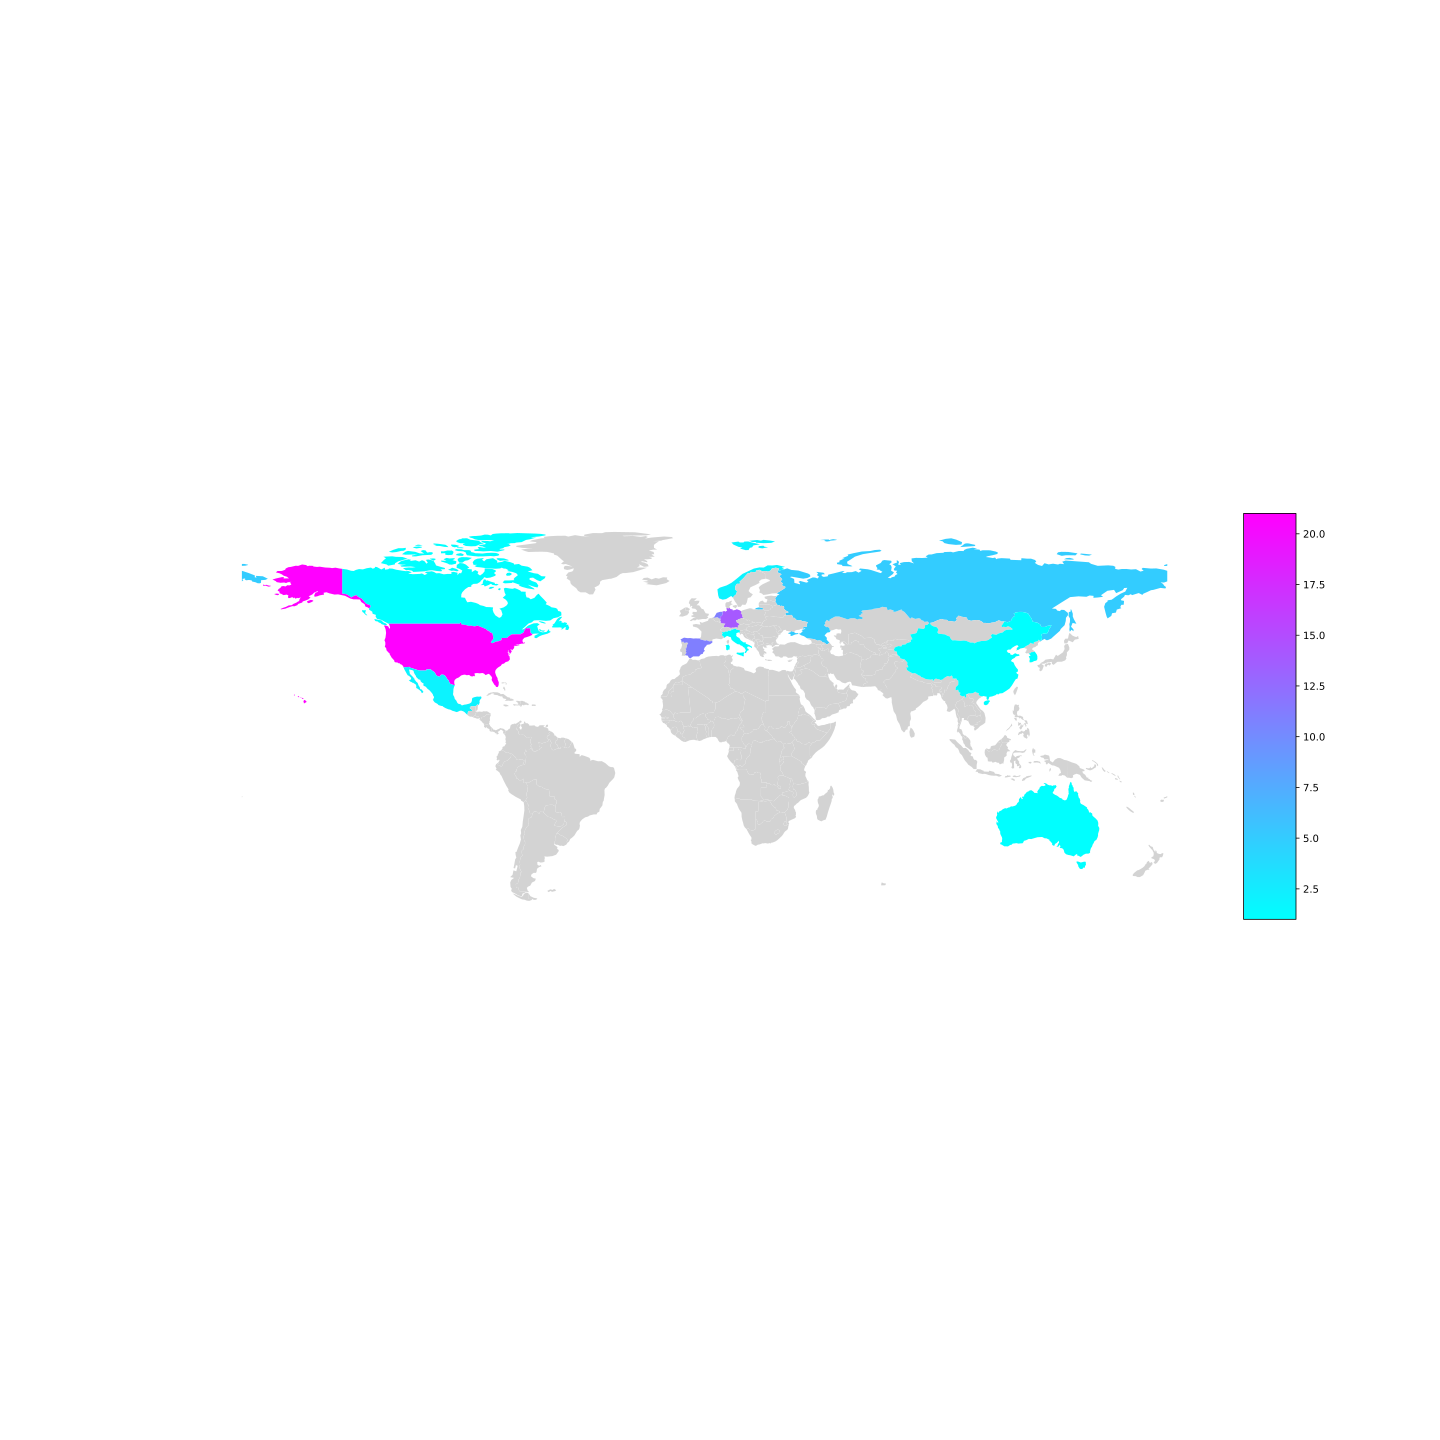
\includegraphics[width=\textwidth]{reports/figures/surveys_per_country.png}
     \caption{Graphic of the number of survey per country}
    \label{fig: surveys_per_country}
\end{figure}

The overview of research topics and the metadata analyses gave a general overview of the research field, which we will expand on in the following sections. We saw an increasing trend in publications and could identify six main research dimensions: data quality, input alternatives, invitation modes, mobile design, mobile participants, online participants, and the meta category reviews. When analysing the metadata of the research articles, we identified several issues that have to be minded when interpreting the results and showcasing current research gaps. We identified an average lag of three years between survey execution and publication, which must be considered when interpreting the results. Other possible biases are caused by the concentration of many articles on a few authors and survey operators. A significant research gap is the unrepresentativeness of the survey populations, which mainly focus on America and Western Europe. An important future research project is to transfer the results identified in the other articles to other world regions. 
